\documentclass[tikz,border=18pt]{standalone}
\usepackage[T1]{fontenc}
\usepackage{helvet}
\renewcommand{\familydefault}{\sfdefault}
\usepackage{amsmath,amssymb}
\usetikzlibrary{calc,positioning,fit,backgrounds,shapes.geometric,shapes.symbols,arrows.meta,decorations.pathreplacing}

% =============================================================================
% MLSYSBOOK CANONICAL COLOR PALETTE
% =============================================================================
\definecolor{BlueLine}{HTML}{006395}
\definecolor{BlueL}{RGB}{209,243,255}
\definecolor{BlueDD}{RGB}{20,50,80}
\definecolor{GreenLine}{HTML}{008F45}
\definecolor{GreenL}{RGB}{219,253,166}
\definecolor{GreenL0}{HTML}{EBF8F2}
\definecolor{OrangeLine}{HTML}{E67817}
\definecolor{OrangeL}{RGB}{254,237,222}
\definecolor{RedLine}{HTML}{D9534F}
\definecolor{RedL}{RGB}{253,226,240}
\definecolor{VioletLine}{HTML}{7E317B}
\definecolor{VioletL}{RGB}{247,215,247}
\definecolor{BrownLine}{RGB}{143,120,116}
\definecolor{BrownL}{RGB}{240,230,225}
\definecolor{GrayLine}{HTML}{64748B}
\definecolor{GrayL}{HTML}{F8FAFC}
\definecolor{CardBorder}{HTML}{CBD5E1}
\definecolor{DarkSlate}{HTML}{0F172A}
\definecolor{ChipBlack}{HTML}{181F2C}
\definecolor{GoldPin}{HTML}{EAB308}

\tikzset{
  >=Stealth,
  font=\sffamily,
  flow_arrow/.style={->, >=Latex, line width=1.3pt},
  bus_arrow/.style={<->, >=Latex, line width=2.0pt},
}

% -----------------------------------------------------------------------------
% PIC DEFINITIONS
% -----------------------------------------------------------------------------

% 1. HBM3e 3D DIE STACK
\tikzset{
  pics/hbm_stack/.style = {
    code = {
      \begin{scope}[local bounding box=HBM, scale=0.92]
        % Base Logic Die
        \draw[fill=BlueLine!35, draw=BlueLine, line width=0.7pt, rounded corners=0.8pt] (0, 0) rectangle (2.6, 0.30);
        \node[font=\bfseries\fontsize{5pt}{6pt}\selectfont, text=BlueDD] at (1.3, 0.15) {Base Logic Die};
        % Micro-bumps
        \foreach \x in {0.2, 0.45, ..., 2.4} {
          \fill[GoldPin] (\x, -0.06) rectangle (\x+0.12, 0);
        }
        % Stacked DRAM Dies (4 layers)
        \foreach \y [count=\idx] in {0.36, 0.62, 0.88, 1.14} {
          \draw[fill=BlueL!60, draw=BlueLine!80, line width=0.5pt, rounded corners=0.6pt] (0.1, \y) rectangle (2.5, \y+0.20);
          \node[font=\fontsize{5pt}{6pt}\selectfont, text=DarkSlate] at (1.3, \y+0.10) {Core DRAM Die \idx};
          % TSV vias
          \fill[GoldPin] (0.28, \y-0.05) rectangle (0.34, \y);
          \fill[GoldPin] (2.26, \y-0.05) rectangle (2.32, \y);
        }
      \end{scope}
    }
  }
}

% 2. DIMM RAM MODULE
\tikzset{
  pics/dimm_ram/.style = {
    code = {
      \begin{scope}[local bounding box=DIMM, scale=0.85]
        % PCB Board
        \draw[fill=GreenLine!22, draw=GreenLine, line width=0.8pt, rounded corners=1.5pt] (0,0) rectangle (4.6, 1.30);
        % Notch at bottom
        \fill[white, draw=GreenLine, line width=0.8pt] (2.0, -0.02) rectangle (2.25, 0.30);
        % DRAM Chips (4 chips)
        \foreach \x in {0.25, 1.1, 2.45, 3.3} {
          \draw[fill=DarkSlate, draw=black, line width=0.4pt, rounded corners=0.5pt] (\x, 0.42) rectangle (\x+0.7, 1.10);
          \draw[white!40, line width=0.3pt] (\x+0.1, 0.90) -- (\x+0.6, 0.90);
        }
        % Gold Pins
        \foreach \x in {0.15, 0.3, ..., 1.85} {
          \fill[GoldPin] (\x, 0.02) rectangle (\x+0.09, 0.15);
        }
        \foreach \x in {2.35, 2.5, ..., 4.35} {
          \fill[GoldPin] (\x, 0.02) rectangle (\x+0.09, 0.15);
        }
        \node[font=\bfseries\fontsize{4.5pt}{5.5pt}\selectfont, text=GreenLine!90!black] at (4.15, 1.18) {DDR5/CXL};
      \end{scope}
    }
  }
}

% 3. TERMINAL WINDOW
\tikzset{
  pics/terminal_win/.style = {
    code = {
      \begin{scope}[local bounding box=TERM, scale=1]
        \draw[fill=DarkSlate, draw=black, line width=0.7pt, rounded corners=2.5pt] (0,0) rectangle (3.0, 1.65);
        % Title bar
        \fill[black!85] (0, 1.35) rectangle (3.0, 1.65);
        \fill[RedLine] (0.2, 1.5) circle (1.2pt);
        \fill[OrangeLine] (0.38, 1.5) circle (1.2pt);
        \fill[GreenLine] (0.56, 1.5) circle (1.2pt);
        \node[font=\fontsize{5.5pt}{6.5pt}\selectfont, text=white!80] at (1.75, 1.5) {\texttt{bash -- sandboxed}};
        % Console Text
        \node[anchor=north west, font=\ttfamily\fontsize{5pt}{6.5pt}\selectfont, text=GreenLine!90!white, inner sep=2pt] at (0.05, 1.30) {\$ pytest tests/};
        \node[anchor=north west, font=\ttfamily\fontsize{5pt}{6.5pt}\selectfont, text=white, inner sep=2pt] at (0.05, 0.95) {5 passed [100\%]};
        \node[anchor=north west, font=\ttfamily\fontsize{5pt}{6.5pt}\selectfont, text=GoldPin, inner sep=2pt] at (0.05, 0.60) {\$ exit 0};
      \end{scope}
    }
  }
}

% 4. BROWSER WINDOW
\tikzset{
  pics/browser_win/.style = {
    code = {
      \begin{scope}[local bounding box=BROWSER, scale=1]
        \draw[fill=white, draw=BlueLine, line width=0.7pt, rounded corners=2.5pt] (0,0) rectangle (3.0, 1.65);
        % Title bar
        \fill[BlueL!30] (0, 1.35) rectangle (3.0, 1.65);
        \fill[RedLine] (0.2, 1.5) circle (1.2pt);
        \fill[OrangeLine] (0.38, 1.5) circle (1.2pt);
        \fill[GreenLine] (0.56, 1.5) circle (1.2pt);
        % URL Bar
        \draw[fill=white, draw=BlueLine!40, line width=0.4pt, rounded corners=1pt] (0.75, 1.38) rectangle (2.9, 1.6);
        \node[font=\fontsize{5pt}{6pt}\selectfont, text=BlueDD] at (1.82, 1.49) {\texttt{https://api.db/query}};
        % DOM elements
        \draw[line width=1.5pt, draw=GrayLine!30] (0.2, 1.15) -- (2.4, 1.15);
        \draw[line width=1.5pt, draw=GrayLine!30] (0.2, 0.92) -- (2.7, 0.92);
        \draw[line width=1.5pt, draw=GrayLine!30] (0.2, 0.69) -- (1.9, 0.69);
        \node[font=\bfseries\fontsize{5.5pt}{6.5pt}\selectfont, text=OrangeLine] at (1.5, 0.35) {Web DOM / MCP Schema};
      \end{scope}
    }
  }
}

% 5. HARDWARE PRIVILEGE RINGS
\tikzset{
  pics/privilege_rings/.style = {
    code = {
      \begin{scope}[local bounding box=RINGS, scale=0.82]
        % Outer Ring (Ring 3: Untrusted SPU Output)
        \draw[fill=OrangeLine!15, draw=OrangeLine, line width=0.8pt] (0,0) circle (1.15cm);
        % Middle Ring (Ring 1: Grammar Filter)
        \draw[fill=GreenLine!15, draw=GreenLine, line width=0.8pt] (0,0) circle (0.78cm);
        % Inner Core (Ring 0: Host OS Kernel)
        \draw[fill=RedLine!20, draw=RedLine, line width=0.9pt] (0,0) circle (0.42cm);
        \node[font=\bfseries\fontsize{4pt}{5pt}\selectfont, text=RedLine, align=center] at (0, 0) {RING 0\\OS};
        \node[font=\bfseries\fontsize{4pt}{5pt}\selectfont, text=GreenLine] at (0, 0.60) {CFG Gate};
        \node[font=\bfseries\fontsize{4pt}{5pt}\selectfont, text=OrangeLine] at (0, 0.96) {Ring 3: Model};
      \end{scope}
    }
  }
}

\begin{document}
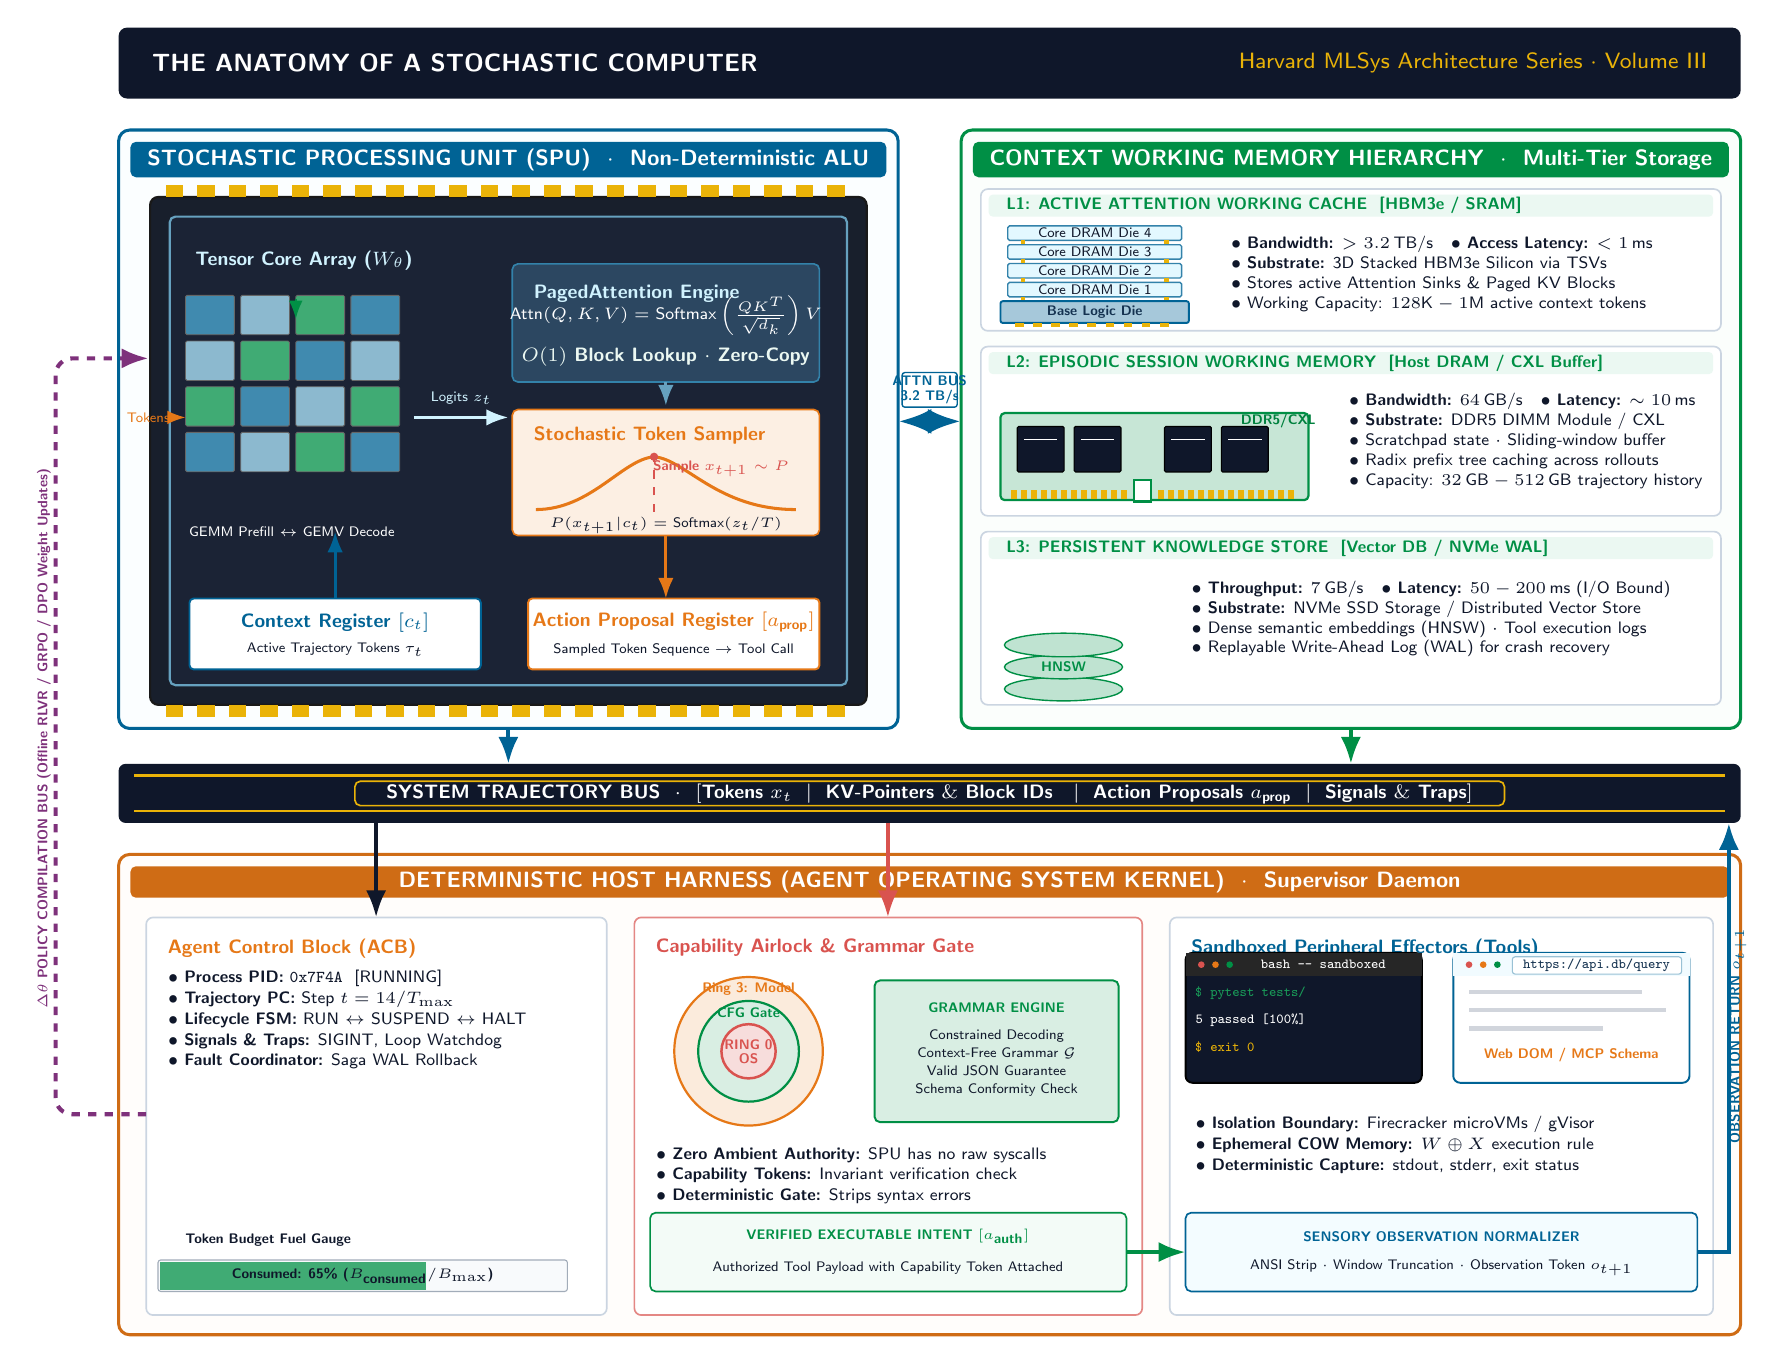
\begin{tikzpicture}[x=1cm, y=1cm]

% =============================================================================
% TOP BANNER
% =============================================================================
\draw[fill=DarkSlate, draw=none, rounded corners=3pt] (0, 15.3) rectangle (20.6, 16.2);
\node[anchor=west, font=\bfseries\small, text=white] at (0.3, 15.75) {
  THE ANATOMY OF A STOCHASTIC COMPUTER
};
\node[anchor=east, font=\footnotesize, text=GoldPin] at (20.3, 15.75) {
  Harvard MLSys Architecture Series $\cdot$ Volume III
};

% =============================================================================
% 1. TOP-LEFT: STOCHASTIC PROCESSING UNIT (SPU)
% =============================================================================
\draw[draw=BlueLine, fill=BlueL!08, line width=1.1pt, rounded corners=4pt] (0, 7.3) rectangle (9.9, 14.9);

% SPU Header Bar
\fill[BlueLine, rounded corners=2pt] (0.15, 14.3) rectangle (9.75, 14.75);
\node[font=\bfseries\footnotesize, text=white] at (4.95, 14.52) {
  STOCHASTIC PROCESSING UNIT (SPU) \ $\cdot$ \ Non-Deterministic ALU
};

% Chip Package Substrate
\draw[fill=ChipBlack, draw=black!90, line width=0.8pt, rounded corners=3pt] (0.4, 7.6) rectangle (9.5, 14.05);

% Pin headers along package top and bottom
\foreach \x in {0.6, 1.0, ..., 9.2} {
  \fill[GoldPin] (\x, 7.45) rectangle (\x+0.22, 7.6);
  \fill[GoldPin] (\x, 14.05) rectangle (\x+0.22, 14.2);
}

% Silicon Die
\draw[fill=DarkSlate!95, draw=BlueLine!60, line width=0.8pt, rounded corners=2pt] (0.65, 7.85) rectangle (9.25, 13.8);

% --- INSIDE SILICON DIE ---

% Column A: Systolic Tensor Core Grid
\begin{scope}[shift={(0.85, 10.1)}]
  \node[anchor=south west, font=\bfseries\scriptsize, text=BlueL] at (0, 2.9) {Tensor Core Array ($W_\theta$)};
  
  % Systolic Cell Grid (4x4)
  \foreach \r in {0,...,3} {
    \foreach \c in {0,...,3} {
      \pgfmathsetmacro{\clr}{int(mod(\r+\c, 3))}
      \ifnum\clr=0 \def\tcol{BlueLine!75} \fi
      \ifnum\clr=1 \def\tcol{BlueLine!45} \fi
      \ifnum\clr=2 \def\tcol{GreenLine!75} \fi
      \draw[fill=\tcol, draw=black!60, line width=0.3pt, rounded corners=0.5pt] 
        (\c*0.7, 2.2-\r*0.58) rectangle (\c*0.7+0.62, 2.2-\r*0.58+0.5);
    }
  }
  % Dataflow Indicators
  \draw[->, >=Latex, line width=0.8pt, draw=OrangeLine] (-0.15, 1.15) -- (0, 1.15) node[left=2pt, font=\fontsize{5pt}{6pt}\selectfont, text=OrangeLine] {Tokens};
  \draw[->, >=Latex, line width=0.8pt, draw=GreenLine] (1.4, 2.65) -- (1.4, 2.4);
  \node[font=\fontsize{5.5pt}{6.5pt}\selectfont, text=white!70] at (1.35, -0.3) {GEMM Prefill $\leftrightarrow$ GEMV Decode};
\end{scope}

% Inter-unit arrow (Tensor core to attention unit)
\draw[flow_arrow, draw=BlueL, line width=1.1pt] (3.75, 11.25) -- (4.95, 11.25);
\node[font=\fontsize{5pt}{6pt}\selectfont, text=BlueL, above=1pt] at (4.35, 11.25) {Logits $z_t$};

% Column B: KV Attention Unit & Stochastic Sampler
\begin{scope}[shift={(5.0, 9.7)}]
  % KV Attention Engine Box
  \draw[fill=BlueDD!90, draw=BlueLine!80, line width=0.6pt, rounded corners=2pt] (0, 2.0) rectangle (3.9, 3.5);
  \node[anchor=north west, font=\bfseries\scriptsize, text=BlueL] at (0.15, 3.35) {PagedAttention Engine};
  \node[font=\fontsize{6pt}{7.5pt}\selectfont, text=white, align=center] at (1.95, 2.65) {
    $\text{Attn}(Q,K,V) = \text{Softmax}\left(\frac{QK^T}{\sqrt{d_k}}\right)V$\\[3pt]
    \textcolor{GreenL0}{\textbf{\scriptsize $O(1)$ Block Lookup $\cdot$ Zero-Copy}}
  };

  % Stochastic Sampler Box
  \draw[fill=OrangeLine!12, draw=OrangeLine, line width=0.6pt, rounded corners=2pt] (0, 0.05) rectangle (3.9, 1.65);
  \node[anchor=north west, font=\bfseries\scriptsize, text=OrangeLine] at (0.15, 1.55) {Stochastic Token Sampler};
  
  % Probability Distribution Curve
  \draw[draw=OrangeLine, line width=1.1pt] 
    (0.3, 0.38) .. controls (1.0, 0.38) and (1.4, 1.02) .. (1.8, 1.05) 
    .. controls (2.2, 1.02) and (2.6, 0.38) .. (3.6, 0.38);
  
  % Sampled Token Line
  \draw[dashed, draw=RedLine, line width=0.8pt] (1.8, 0.35) -- (1.8, 1.05);
  \fill[RedLine] (1.8, 1.05) circle (1.5pt);
  \node[font=\bfseries\fontsize{4.5pt}{5.5pt}\selectfont, text=RedLine] at (2.65, 0.90) {Sample $x_{t+1} \sim P$};
  \node[font=\fontsize{5.5pt}{6.5pt}\selectfont, text=DarkSlate] at (1.95, 0.18) {$P(x_{t+1}|c_t) = \text{Softmax}(z_t / T)$};
\end{scope}

% Internal Connection from Attention Engine down to Sampler
\draw[flow_arrow, draw=BlueLine!60, line width=1.0pt] (6.95, 11.7) -- (6.95, 11.4);

% Bottom SPU Registers
\draw[fill=white, draw=BlueLine, line width=0.7pt, rounded corners=1.5pt] (0.9, 8.05) rectangle (4.6, 8.95);
\node[font=\bfseries\scriptsize, text=BlueLine] at (2.75, 8.65) {Context Register $[c_t]$};
\node[font=\fontsize{5.5pt}{6.5pt}\selectfont, text=DarkSlate] at (2.75, 8.3) {Active Trajectory Tokens $\tau_t$};

\draw[fill=white, draw=OrangeLine, line width=0.7pt, rounded corners=1.5pt] (5.2, 8.05) rectangle (8.9, 8.95);
\node[font=\bfseries\scriptsize, text=OrangeLine] at (7.05, 8.65) {Action Proposal Register $[a_{\text{prop}}]$};
\node[font=\fontsize{5.5pt}{6.5pt}\selectfont, text=DarkSlate] at (7.05, 8.3) {Sampled Token Sequence $\to$ Tool Call};

\draw[flow_arrow, draw=BlueLine, line width=1.0pt] (2.75, 8.95) -- (2.75, 9.8);
\draw[flow_arrow, draw=OrangeLine, line width=1.0pt] (6.95, 9.75) -- (6.95, 8.95);

% =============================================================================
% 2. TOP-RIGHT: CONTEXT & WORKING MEMORY HIERARCHY
% =============================================================================
\draw[draw=GreenLine, fill=GreenL0!20, line width=1.1pt, rounded corners=4pt] (10.7, 7.3) rectangle (20.6, 14.9);

% Memory Header Bar
\fill[GreenLine, rounded corners=2pt] (10.85, 14.3) rectangle (20.45, 14.75);
\node[font=\bfseries\footnotesize, text=white] at (15.65, 14.52) {
  CONTEXT WORKING MEMORY HIERARCHY \ $\cdot$ \ Multi-Tier Storage
};

% --- TIER 1: L1 ACTIVE ATTENTION WORKING CACHE (HBM3e) ---
\draw[fill=white, draw=CardBorder, line width=0.6pt, rounded corners=2.5pt] (10.95, 12.35) rectangle (20.35, 14.15);
\fill[GreenL0, rounded corners=1.5pt] (11.05, 13.80) rectangle (20.25, 14.08);
\node[anchor=west, font=\bfseries\fontsize{6pt}{7pt}\selectfont, text=GreenLine] at (11.15, 13.94) {
  L1: ACTIVE ATTENTION WORKING CACHE \ [HBM3e / SRAM]
};
\pic at (11.2, 12.45) {hbm_stack};
\node[anchor=north west, font=\fontsize{5.8pt}{7.2pt}\selectfont, text=DarkSlate, align=left] at (14.0, 13.68) {
  $\bullet$ \textbf{Bandwidth:} $>3.2\,\text{TB/s} \quad \bullet$ \textbf{Access Latency:} $<1\,\text{ms}$\\
  $\bullet$ \textbf{Substrate:} 3D Stacked HBM3e Silicon via TSVs\\
  $\bullet$ Stores active Attention Sinks \& Paged KV Blocks\\
  $\bullet$ Working Capacity: $128\text{K} - 1\text{M}$ active context tokens
};

% --- TIER 2: L2 EPISODIC SESSION RAM (Host DRAM) ---
\draw[fill=white, draw=CardBorder, line width=0.6pt, rounded corners=2.5pt] (10.95, 10.0) rectangle (20.35, 12.15);
\fill[GreenL0, rounded corners=1.5pt] (11.05, 11.80) rectangle (20.25, 12.08);
\node[anchor=west, font=\bfseries\fontsize{6pt}{7pt}\selectfont, text=GreenLine] at (11.15, 11.94) {
  L2: EPISODIC SESSION WORKING MEMORY \ [Host DRAM / CXL Buffer]
};
\pic at (11.2, 10.2) {dimm_ram};
\node[anchor=north west, font=\fontsize{5.8pt}{7.2pt}\selectfont, text=DarkSlate, align=left] at (15.5, 11.68) {
  $\bullet$ \textbf{Bandwidth:} $64\,\text{GB/s} \quad \bullet$ \textbf{Latency:} $\sim 10\,\text{ms}$\\
  $\bullet$ \textbf{Substrate:} DDR5 DIMM Module / CXL\\
  $\bullet$ Scratchpad state $\cdot$ Sliding-window buffer\\
  $\bullet$ Radix prefix tree caching across rollouts\\
  $\bullet$ Capacity: $32\,\text{GB} - 512\,\text{GB}$ trajectory history
};

% --- TIER 3: L3 PERSISTENT ARCHIVAL STORAGE ---
\draw[fill=white, draw=CardBorder, line width=0.6pt, rounded corners=2.5pt] (10.95, 7.6) rectangle (20.35, 9.8);
\fill[GreenL0, rounded corners=1.5pt] (11.05, 9.45) rectangle (20.25, 9.73);
\node[anchor=west, font=\bfseries\fontsize{6pt}{7pt}\selectfont, text=GreenLine] at (11.15, 9.59) {
  L3: PERSISTENT KNOWLEDGE STORE \ [Vector DB / NVMe WAL]
};
% Disk Platter Icon
\begin{scope}[shift={(12.0, 7.8)}]
  \foreach \h in {0, 0.28, 0.56} {
    \draw[fill=GreenLine!25, draw=GreenLine, line width=0.5pt] (0, \h) ellipse (0.75cm and 0.15cm);
  }
  \node[font=\bfseries\fontsize{5.5pt}{6.5pt}\selectfont, text=GreenLine] at (0, 0.28) {HNSW};
\end{scope}
\node[anchor=north west, font=\fontsize{5.8pt}{7.2pt}\selectfont, text=DarkSlate, align=left] at (13.5, 9.30) {
  $\bullet$ \textbf{Throughput:} $7\,\text{GB/s} \quad \bullet$ \textbf{Latency:} $50-200\,\text{ms}$ (I/O Bound)\\
  $\bullet$ \textbf{Substrate:} NVMe SSD Storage / Distributed Vector Store\\
  $\bullet$ Dense semantic embeddings (HNSW) $\cdot$ Tool execution logs\\
  $\bullet$ Replayable Write-Ahead Log (WAL) for crash recovery
};

% =============================================================================
% INTERCONNECT: HIGH-SPEED ATTENTION BUS
% =============================================================================
\draw[bus_arrow, draw=BlueLine] (9.9, 11.2) -- (10.7, 11.2);
\draw[fill=white, draw=BlueLine, line width=0.5pt, rounded corners=1pt] (9.95, 11.38) rectangle (10.65, 11.82);
\node[font=\bfseries\fontsize{4.5pt}{5.5pt}\selectfont, text=BlueLine, align=center] at (10.3, 11.6) {ATTN BUS\\3.2 TB/s};

% =============================================================================
% 3. MIDDLE: SYSTEM TRAJECTORY & CONTROL BUS
% =============================================================================
\fill[DarkSlate, rounded corners=2.5pt] (0, 6.1) rectangle (20.6, 6.85);

% Parallel Copper Bus Lines
\draw[GoldPin, line width=0.9pt] (0.2, 6.25) -- (20.4, 6.25);
\draw[GoldPin, line width=0.9pt] (0.2, 6.7) -- (20.4, 6.7);

% Clean Bus Title Badge
\draw[fill=DarkSlate, draw=GoldPin, line width=0.6pt, rounded corners=2pt] (3.0, 6.32) rectangle (17.6, 6.63);
\node[font=\bfseries\scriptsize, text=white] at (10.3, 6.47) {
  SYSTEM TRAJECTORY BUS \ $\cdot$ \ $[\text{Tokens } x_t \ \mid \ \text{KV-Pointers } \& \ \text{Block IDs } \ \mid \ \text{Action Proposals } a_{\text{prop}} \ \mid \ \text{Signals } \& \ \text{Traps}]$
};

% Bus Taps
\draw[flow_arrow, draw=BlueLine, line width=1.5pt] (4.95, 7.3) -- (4.95, 6.85);
\draw[flow_arrow, draw=GreenLine, line width=1.5pt] (15.65, 7.3) -- (15.65, 6.85);

% =============================================================================
% 4. BOTTOM TIER: DETERMINISTIC HOST HARNESS (AGENT OS KERNEL)
% =============================================================================
\draw[draw=OrangeLine!90!black, fill=OrangeL!12, line width=1.1pt, rounded corners=4pt] (0, -0.4) rectangle (20.6, 5.7);

% Host Harness Header Bar
\fill[OrangeLine!90!black, rounded corners=2pt] (0.15, 5.15) rectangle (20.45, 5.55);
\node[font=\bfseries\footnotesize, text=white] at (10.3, 5.35) {
  DETERMINISTIC HOST HARNESS (AGENT OPERATING SYSTEM KERNEL) \ $\cdot$ \ Supervisor Daemon
};

% --- BLOCK 4A: AGENT CONTROL BLOCK (ACB) & SCHEDULER (Left) ---
\draw[fill=white, draw=CardBorder, line width=0.6pt, rounded corners=2.5pt] (0.35, -0.15) rectangle (6.2, 4.9);
\node[anchor=north west, font=\bfseries\scriptsize, text=OrangeLine] at (0.5, 4.75) {Agent Control Block (ACB)};

\node[anchor=north west, font=\fontsize{6pt}{7.5pt}\selectfont, text=DarkSlate, align=left] at (0.5, 4.35) {
  $\bullet$ \textbf{Process PID:} \texttt{0x7F4A} \ [RUNNING]\\
  $\bullet$ \textbf{Trajectory PC:} Step $t = 14 / T_{\max}$\\
  $\bullet$ \textbf{Lifecycle FSM:} $\text{RUN} \leftrightarrow \text{SUSPEND} \leftrightarrow \text{HALT}$\\
  $\bullet$ \textbf{Signals \& Traps:} SIGINT, Loop Watchdog\\
  $\bullet$ \textbf{Fault Coordinator:} Saga WAL Rollback
};

% Token Budget Fuel Gauge
\begin{scope}[shift={(0.5, 0.15)}]
  \node[font=\bfseries\fontsize{5.5pt}{6.5pt}\selectfont, text=DarkSlate] at (1.4, 0.65) {Token Budget Fuel Gauge};
  \draw[draw=GrayLine!60, fill=GrayL, line width=0.4pt, rounded corners=1pt] (0, 0) rectangle (5.2, 0.4);
  \fill[GreenLine!75] (0.02, 0.02) rectangle (3.4, 0.38);
  \node[font=\bfseries\fontsize{5pt}{6pt}\selectfont, text=DarkSlate] at (2.6, 0.2) {Consumed: 65\% ($B_{\text{consumed}} / B_{\max}$)};
\end{scope}

% --- BLOCK 4B: PRIVILEGE SEPARATION & GRAMMAR AIRLOCK (Center) ---
\draw[fill=white, draw=RedLine!70, line width=0.6pt, rounded corners=2.5pt] (6.55, -0.15) rectangle (13.0, 4.9);
\node[anchor=north west, font=\bfseries\scriptsize, text=RedLine] at (6.7, 4.75) {Capability Airlock \& Grammar Gate};

% Hardware Privilege Rings Icon
\pic at (8.0, 3.2) {privilege_rings};

% Grammar Engine Box
\begin{scope}[shift={(9.6, 2.3)}]
  \draw[fill=GreenLine!15, draw=GreenLine, line width=0.7pt, rounded corners=2pt] (0, 0) rectangle (3.1, 1.8);
  \node[font=\bfseries\fontsize{5.5pt}{6.5pt}\selectfont, text=GreenLine, align=center] at (1.55, 1.45) {GRAMMAR ENGINE};
  \node[font=\fontsize{5pt}{6.5pt}\selectfont, text=DarkSlate, align=center] at (1.55, 0.75) {
    Constrained Decoding\\
    Context-Free Grammar $\mathcal{G}$\\
    Valid JSON Guarantee\\
    Schema Conformity Check
  };
\end{scope}

\node[anchor=north west, font=\fontsize{6pt}{7.5pt}\selectfont, text=DarkSlate, align=left] at (6.7, 2.1) {
  $\bullet$ \textbf{Zero Ambient Authority:} SPU has no raw syscalls\\
  $\bullet$ \textbf{Capability Tokens:} Invariant verification check\\
  $\bullet$ \textbf{Deterministic Gate:} Strips syntax errors
};

% Verified Action Register
\draw[fill=GreenL0!60, draw=GreenLine, line width=0.6pt, rounded corners=2pt] (6.75, 0.15) rectangle (12.8, 1.15);
\node[font=\bfseries\fontsize{5.5pt}{6.5pt}\selectfont, text=GreenLine] at (9.77, 0.85) {VERIFIED EXECUTABLE INTENT $[a_{\text{auth}}]$};
\node[font=\fontsize{5pt}{6pt}\selectfont, text=DarkSlate] at (9.77, 0.45) {Authorized Tool Payload with Capability Token Attached};

% --- BLOCK 4C: SANDBOXED PERIPHERAL EFFECTORS (Right) ---
\draw[fill=white, draw=CardBorder, line width=0.6pt, rounded corners=2.5pt] (13.35, -0.15) rectangle (20.25, 4.9);
\node[anchor=north west, font=\bfseries\scriptsize, text=BlueLine] at (13.5, 4.75) {Sandboxed Peripheral Effectors (Tools)};

% Terminal & Browser Pics
\pic at (13.55, 2.8) {terminal_win};
\pic at (16.95, 2.8) {browser_win};

\node[anchor=north west, font=\fontsize{6pt}{7.5pt}\selectfont, text=DarkSlate, align=left] at (13.55, 2.5) {
  $\bullet$ \textbf{Isolation Boundary:} Firecracker microVMs / gVisor\\
  $\bullet$ \textbf{Ephemeral COW Memory:} $W \oplus X$ execution rule\\
  $\bullet$ \textbf{Deterministic Capture:} stdout, stderr, exit status
};

% Sensory Observation Normalizer
\draw[fill=BlueL!25, draw=BlueLine, line width=0.6pt, rounded corners=2pt] (13.55, 0.15) rectangle (20.05, 1.15);
\node[font=\bfseries\fontsize{5.5pt}{6.5pt}\selectfont, text=BlueLine] at (16.8, 0.85) {SENSORY OBSERVATION NORMALIZER};
\node[font=\fontsize{5pt}{6pt}\selectfont, text=DarkSlate] at (16.8, 0.45) {ANSI Strip $\cdot$ Window Truncation $\cdot$ Observation Token $o_{t+1}$};

% Bus connections to bottom tier
\draw[flow_arrow, draw=DarkSlate, line width=1.5pt] (3.27, 6.1) -- (3.27, 4.9);
\draw[flow_arrow, draw=RedLine, line width=1.5pt] (9.77, 6.1) -- (9.77, 4.9);
\draw[flow_arrow, draw=GreenLine, line width=1.5pt] (12.8, 0.65) -- (13.55, 0.65);

% Observation Return Bus
\draw[flow_arrow, draw=BlueLine, line width=1.5pt] 
  (20.05, 0.65) -- (20.45, 0.65) -- (20.45, 6.1);
\node[font=\bfseries\fontsize{5pt}{6pt}\selectfont, text=BlueLine, rotate=90] at (20.57, 3.4) {OBSERVATION RETURN $o_{t+1}$};

% =============================================================================
% 5. OFFLINE TRAJECTORY LEARNING & COMPILATION LOOP (OUTER LEFT)
% =============================================================================
\draw[dashed, ->, >=Latex, draw=VioletLine, line width=1.5pt, rounded corners=6pt] 
  (0.35, 2.4) -- (-0.8, 2.4) -- (-0.8, 12.0) -- (0.38, 12.0);
\node[font=\bfseries\fontsize{5.5pt}{6.5pt}\selectfont, text=VioletLine, rotate=90, align=center] at (-0.95, 7.2) {
  $\Delta\theta$ POLICY COMPILATION BUS (Offline RLVR / GRPO / DPO Weight Updates)
};

\end{tikzpicture}
\end{document}
